\scanpage{43}
\diagram{\begin{tikzcd}[ampersand replacement=\&, column sep=huge,row sep=small]
\mathcal H^1(X;A)\arrow[d,no head]\&\operatorname{Ext}^1(A,\operatorname{Pic})\\
\text{\unsure{pt singuliers}}\&
\end{tikzcd}}
\[
\boxed{\mathcal H^1(X,G)\simeq\operatorname{Hom}(D(G),\underline{\operatorname{Pic}}_X)}
\]
\figure{\begin{tikzpicture}[x=1cm,y=1cm]
\draw (0,0) .. controls (-.7,.7) and (.5,1.6) .. (1.1,1.5) .. controls (1.2,.7) and (.3,-.3) .. (0,0);
\draw (-.12,.65) .. controls (.2,1.35) and (.7,1.65) .. (1.1,1.5);
\fill (1.1,1.5) circle (.045);\node at (.71,1.2) {$-$};
\draw (2,1.2) .. controls (2.1,1.8) and (2.6,2.2) .. (2.8,2.15)
.. controls (3.4,2.4) and (3.35,.75) .. (2.8,1.05)
.. controls (2.45,1.2) and (2.65,2.7) .. (3.3,2.8);
\fill (2.8,2.15) circle (.045);
\end{tikzpicture}}
\[\mathcal H^i(X,D(G))\simeq\operatorname{Ext}^i(G,\underline{\operatorname{Pic}}_X)\]
\[\operatorname{Ext}^i_X(f^!(G),G_m)\simeq\operatorname{Ext}^i_Y(G,f_!(G_m))\]
\[
\boxed{\underline{\operatorname{Ext}}^i_X(f^*(G_{\bullet}),H^{\bullet})\simeq
\underline{\operatorname{Ext}}^i_Y(G_{\bullet},f_!(H^{\bullet}))}
\]
\diagram{\begin{tikzcd}[ampersand replacement=\&]X\arrow[d,"f"']\\Y\end{tikzcd}}
\[H=G_m\]
\figure{\begin{tikzpicture}[baseline=(d.base)]
\node[inner sep=0pt] (d) {$\underline{\operatorname{Ext}}^i_X(\underset{\inserted{\unsure{R}}}{f^*}(G),G_m)
\simeq\underline{\operatorname{Ext}}^i_Y(G,
\begin{tikzpicture}[baseline=(p.base)]
\node[draw,ellipse,inner xsep=5pt,inner ysep=12pt] (p) {$\underline{\operatorname{Pic}}^{\bullet}_{X/Y}$};
\node[anchor=south] at (p.north) {\unsure{les supérieurs}};
\draw ([xshift=-1pt,yshift=3pt]p.south)--++(0,-8mm);\draw ([xshift=1pt,yshift=3pt]p.south)--++(0,-8mm);
\end{tikzpicture})$};
\node[anchor=north] at ([xshift=-28mm,yshift=-2mm]d.south) {$\deleted{\unsure{R\Gamma(X,}}$};
\draw ([xshift=-13mm,yshift=2mm]d.south)--++(.02,-.7)--++(.16,-.4);
\draw ([xshift=-11mm,yshift=2mm]d.south)--++(.01,-.7)--++(-.03,-.4);
\end{tikzpicture}}
\[
\boxed{G\ \text{\uline{affine}},\ \text{alors}\quad H^i(X,D(G))\Longleftarrow
\deleted{\unsure{E}}\operatorname{Ext}^{\unsure{i|p}}(G,\operatorname{Pic}^{\unsure{(q)|(1)}}_{X/Y})}
\]
\[
\diagram{\begin{array}{rll}
i=0&H^0(X,D(G))=&\deleted{\operatorname{Hom}}D(G)\\
i=1&H^1(X,D(G))=&\deleted{\unsure{\operatorname{Ext}}}\operatorname{Hom}(G,\operatorname{Pic}^{(1)})\\
i=2&H^2(X,D(G))\underset{!}{\neq}&\operatorname{Ext}^1(G,\operatorname{Pic}^{(1)}_{X/Y})+\operatorname{Hom}(G,\underline{\operatorname{Pic}}^{\unsure{(2)}}_{\unsure{X}})
\end{array}}
\]
\figure{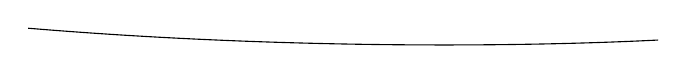
\begin{tikzpicture}\draw (0,.15)..controls (3,-.1) and (6,-.1)..(8,0);\end{tikzpicture}}
$G$ abélien, alors \deleted{$\unsure{H}$}
\[H^{i-1}(X,G')\Longleftarrow\operatorname{Ext}^{\unsure{p}}_{\unsure{q|g}}(G,\operatorname{Pic}^{q}_{X/Y})\]
\[
\diagram{\begin{array}{rl}i=0&0\longrightarrow0\\i=1&H^0(X,G')=\end{array}}
\]
\margin{42}
